\chapter{Future prospects}

\begin{bf}
  \author{Leon V. E. Koopmans (Kapteyn Astronomical Institute), Gianni Bernardi (INAF-IRA \& Rhodes University)}\\
  
Abstract\\
\end{bf}

This chapter discusses some important things

\section{Forthcoming interferometric ground based instruments and upgrades}

\subsection{The Hydrogen Epoch of Reionization Array - 1 page}
\begin{figure}[]
\begin{center}
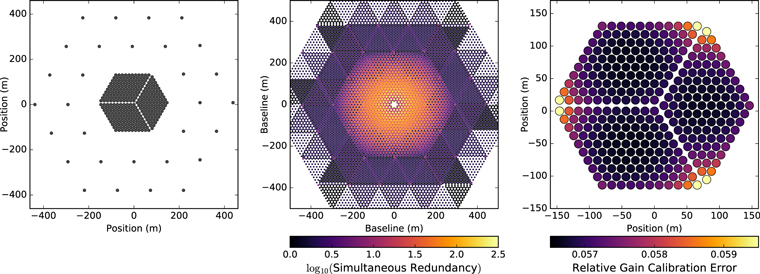
\includegraphics[width=1.\textwidth]{Koopmans_Bernardi/hera_layout}
\end{center}
\caption{HERA antenna layout}
\label{fig:fig_hera}
\end{figure}
The Hydrogen Epoch of Reionization Array (HERA) is an array currently under construction in the Karoo reserve area in South Africa - following the conclusion of the PAPER experiment. HERA is built following the approach used for PAPER: a highly redundant array to maximize the sensitivity on a number of power spectrum modes measured using the avoidance approach. In order to increase the sensitivity with respect to PAPER, it employs 14 m diameter dishes that, in the final configuration, will be densely packed in a highly redundant hexagonal array configuration of $\sim 350$ m diameter. 
HERA is built with the purpose to provide a complete statistical characterization of cosmic reionization: its high brightness sensitivity configuration leads to a significant ($> 10$) power spectrum detection in the $0.2 < k < 0.4$ Mpc-1 range throughout reionization (i.e., 6 < z < 12; Pober et al., 2014; deBoer et al., 2017), fully constraining the evolution of the IGM neutral Hydrogen fraction. As the avoidance approach does not take advantage of foreground modeling, particular attention was paid to prevent the instrumental frequency response from corrupting intrinsically smooth foregrounds (Ewall-Wice et al., 2015; Patra et al., 2017).
HERA is currently under construction, with more than 200 dishes deployed and science observations routinely carried out (Carilli et al. 2018, Kohn et al. 2019). New feeds that extend the sensitivity to the 50-250 MHz (i.e. enabling observations of the Cosmic Dawn) are currently deployed for testing.
In summary, HERA is planned to deliver a complete characterization of cosmic reionization and to attempt the detection of the Cosmic Dawn. Given its redundant configuration, imaging capabilities remain limited and will be the target of a next generation experiment.


\subsection{The Large aperture Experiment to detect the Dark Ages - 1 page}
\begin{figure}[]
\begin{center}
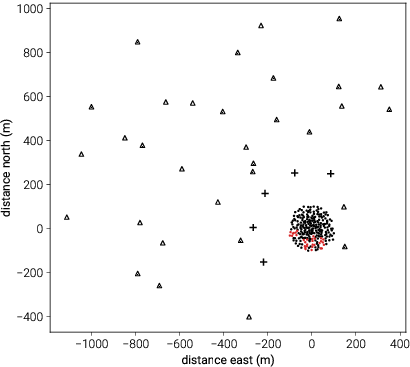
\includegraphics[width=1.\textwidth]{Koopmans_Bernardi/lwa_layout}
\end{center}
\caption{LEDA antenna layout}
\label{fig:fig_leda}
\end{figure}
The Large aperture Experiment to detect the Dark Ages (LEDA) is located in Owens Valley, California. It operates in the 30-88 MHz frequency range corresponding to $15 < z < 46$, therefore seeking to detect the 21 cm signal from the Cosmic Dawn. It is equipped to attempt the measurement of both the global signal via individual dipoles equipped with custom-built calibration sources and 21 cm fluctuations via an array of 256 dipoles. Dipoles are pseudo randomly distributed to achieve an essentially filled array within a ~200 m diameter core, providing excellent imaging capabilities to Galactic diffuse emission - the brightest foreground component. The LEDA approach to measure the 21 cm signal can be versatile, allowing to image and subtract foregrounds but also to isolate them in the power spectrum domain without any specific modeling. Current simulations shows that if IGM heating occurs efficiently at z ~ 16, LEDA would be able to detect the 21 cm power spectrum at $k \sim 0.1$ Mpc-1 with a ~10 signal to noise ratio in 3000 hours. First observations have set a 108 (mK)2 upper limits on the 21 cm power spectrum at k = 0.1 Mpc-1 at z = 18.4 (Eastwood et al. 2019)


\subsection{MWA phase II - Bernardi - 1 page}





\section{Forthcoming Global Signal Experiments}

\subsection{EDGES - Bernardi - 0.5 page}
\begin{figure}[]
\begin{center}
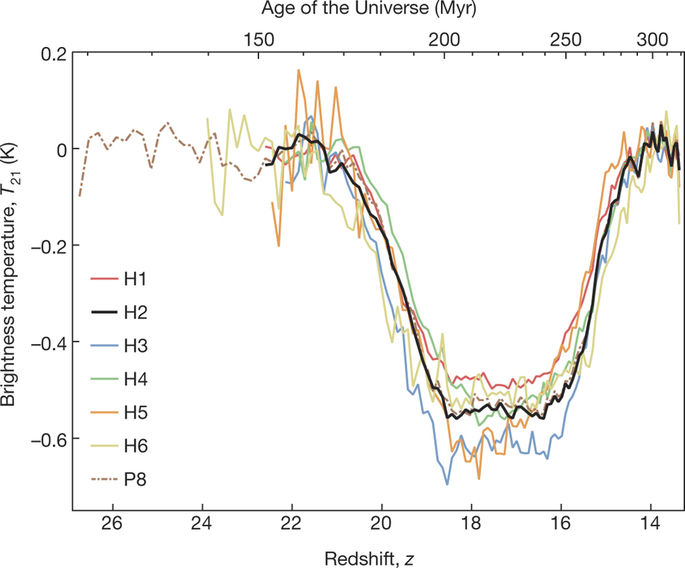
\includegraphics[width=1.\textwidth]{Koopmans_Bernardi/edges_trough}
\end{center}
\caption{EDGES}
\label{fig:fig_edges}
\end{figure}

\subsection{LEDA - Bernardi - 0.5 page}
\begin{figure}[]
\begin{center}
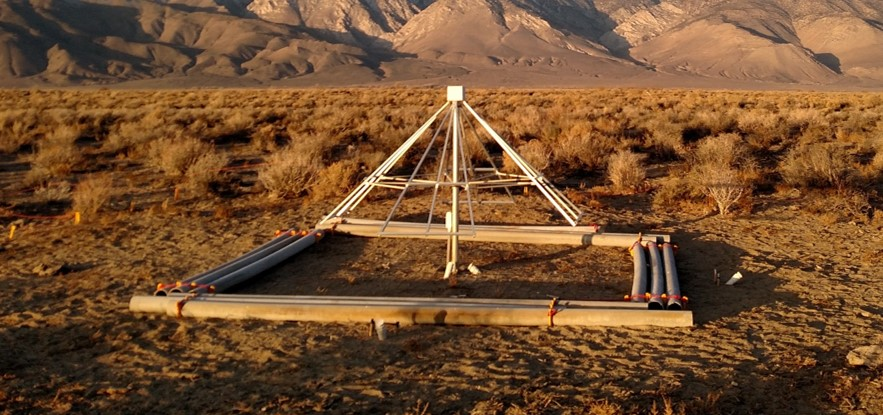
\includegraphics[width=1.\textwidth]{Koopmans_Bernardi/leda_dipole}
\end{center}
\caption{LEDA dipole}
\label{fig:fig_leda_dipole}
\end{figure}




\section{A Section}

Lorem ipsum dolor sit amet, consectetur adipiscing elit. Duis eu egestas erat. Maecenas tincidunt lacinia tincidunt. Mauris id lectus nec neque feugiat condimentum vitae at diam. In vel orci nunc, non commodo mauris. Vivamus ipsum enim, vulputate quis pharetra non, molestie quis felis. Vivamus porttitor placerat turpis at accumsan. Nunc tortor velit, faucibus a rhoncus nec, blandit non elit. Nam consectetur lectus eu nisi blandit dapibus rhoncus dui tempus. Mauris fermentum dolor vel ipsum vulputate sit amet ultricies tortor lacinia. Donec ut nibh erat. Morbi nec mi ante. Integer nec vestibulum diam. Donec tincidunt pellentesque quam, ut interdum mauris venenatis condimentum. Nam condimentum, augue in aliquet gravida, neque dui elementum eros, id semper eros purus sed felis. Curabitur in justo sit amet sapien ultrices hendrerit at quis nibh. Quisque iaculis pulvinar tincidunt. 
\begin{eqnarray}
C(12) &= &\left[\overrightarrow{\pi}\cdot\overrightarrow{\phi}(x+r)\right] \nonumber \\ 
&\approx& 1-\mathrm{const}\frac{r^2}{L^2}\int_r^L\frac{x\rmd x}{x^2} + \cdots \nonumber  \\
&\approx& 1-\mathrm{const}\frac{r^2}{L^2}\ln\frac{x\rmd x}{x^2} + \cdots .\label{brokenlongeqn}
\end{eqnarray}

Aenean tellus risus, porta sit amet porta vitae, tincidunt ut felis. Class aptent taciti sociosqu ad litora torquent per conubia nostra, per inceptos himenaeos. Vestibulum ante ipsum primis in faucibus orci luctus et ultrices posuere cubilia Curae; Phasellus pulvinar placerat velit auctor egestas. Vivamus euismod fringilla tincidunt. Sed ut magna felis, id sollicitudin nunc. Quisque a dui eu erat consectetur egestas a quis justo. Aenean euismod congue diam, vel posuere urna fermentum sit amet. Lorem ipsum dolor sit amet, consectetur adipiscing elit. Mauris faucibus lacus eget est mollis auctor. Donec at nibh ligula, et posuere massa. Phasellus quis leo diam \cite{diamantaras1996pcn}.
Donec aliquam blandit risus, eu venenatis ante euismod eu. Curabitur cursus justo id arcu condimentum feugiat. Integer sapien urna, vulputate et adipiscing nec, convallis et justo. Suspendisse in ipsum at felis ornare interdum \cite{tulone2006pts},

\begin{figure}[]
\begin{center}
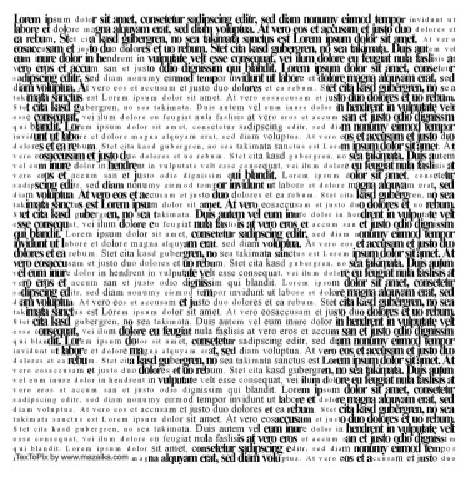
\includegraphics[width=0.5\textwidth]{Koopmans_Bernardi/01x01-eps-converted-to}
\end{center}
\caption{This is figure 1 in chapter 1.}
\end{figure}

\paragraph{Cras adipiscing} sagittis nunc vel luctus. Suspendisse volutpat augue quis erat semper consequat dignissim tellus euismod. Morbi hendrerit, tellus id aliquam iaculis, nibh leo tincidunt eros, vitae varius ligula felis in mi.

\begin{table}
\caption{Greek Letters.}
\begin{center}
\begin{tabular}{llllllll}
\hline
$\alpha $  & $ \beta $  & $ \gamma $  & $ \delta $  & $ \epsilon $  & $ \varepsilon $  & $ \zeta $  & $ \eta $ \\
 $ \theta $  &  $ \vartheta $  &  $ \gamma $  &  $ \kappa $  &  $ \lambda $  &  $ \mu $  &  $ \nu $  &  $ \xi $ \\
 $ o $  &  $ \pi $  &  $ \varpi $  &  $ \rho $  &  $ \varrho $  &  $ \sigma $  &  $ \varsigma $  &  $$ \\
 $ \tau $  &  $ \upsilon $  &  $ \phi$ &  $ \varphi $  &  $ \chi $  &  $ \psi $  &  $ \omega$  &  $ $ \\
 &  &  &  &  &  &  & \\
$ \Gamma $  & $ \Delta $  & $ \Theta $  &  $ \Lambda $  &  $ \Xi $  &  $ \Pi $  &  $ \Sigma $  & $ \Upsilon $ \\
 $ \Phi$ &  $ \Psi $  &  $ \Omega $  &  &  &  &  &\\
\hline
\end{tabular}
\end{center}\end{table}

%\begin{figure}[]
%\begin{center}
%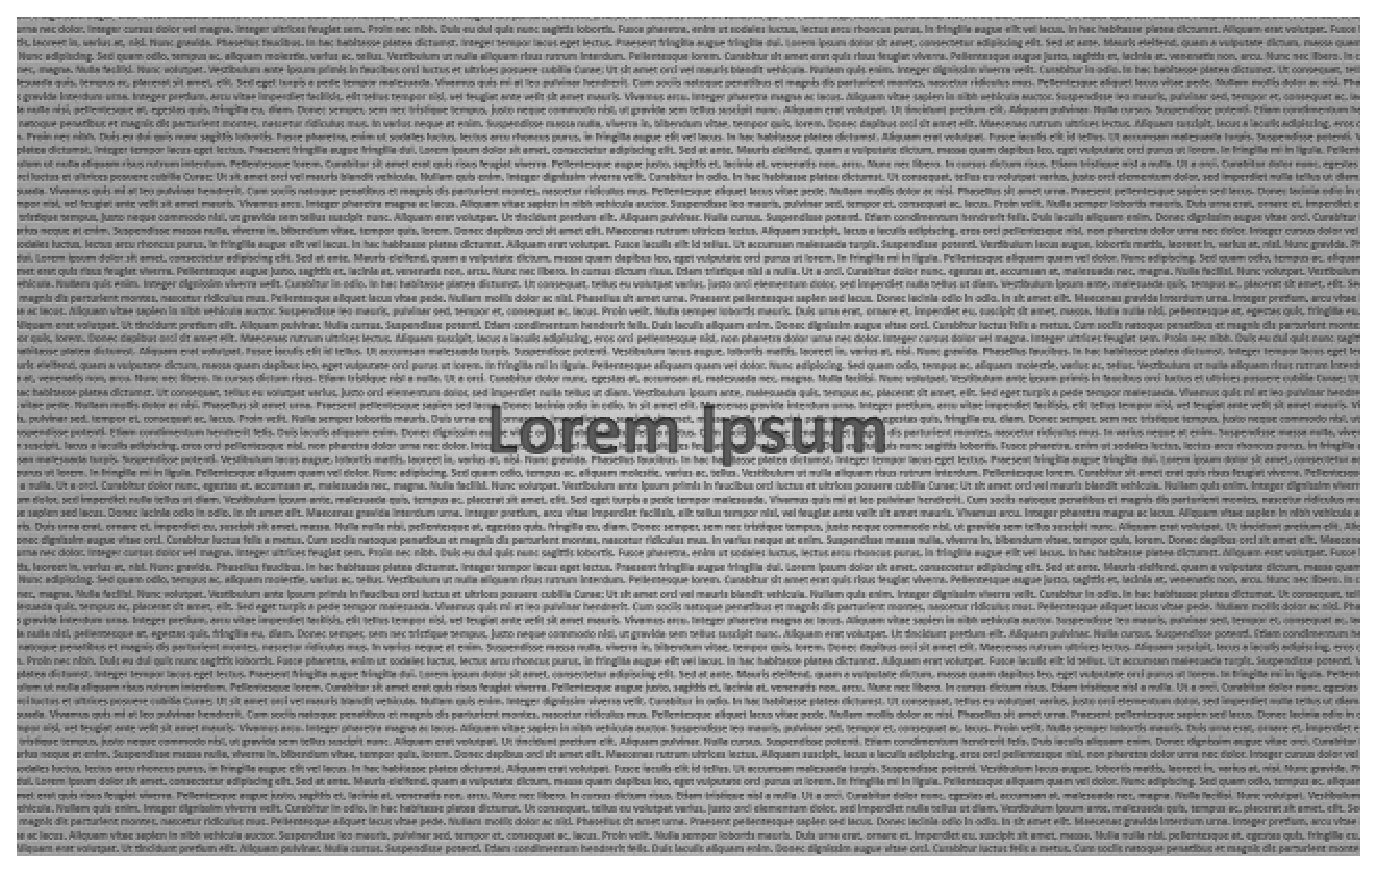
\includegraphics[width=0.6\textwidth]{Koopmans_Bernardi/01x02}
%\end{center}
%\caption{This is figure 2 in chapter 1.}
%\end{figure}


\bibliographystyle{plain}
\bibliography{Koopmans_Bernardi/References}


